\newpage
\section{Resultados}
\indent Para probar el protocolo, armamos archivos de 1kb, 5kb, 10kb, 50kb, 100kb, 200kb y
500kb. El servidor y el cliente se encuentran en distintos host en la misma LAN sobre Wi-Fi la cual presenta un RTT de aproximadamente 2ms entre ambos hosts. Para
tomar los tiempos y comprobar el correcto funcionamiento del protocolo, usamos
el wireshark.\\
\indent Para tener mediciones mas aproximadas a la realidad, tomamos el promedio de 10 mediciones.\\

\subsection{Tiempo de transmisión}
\indent En este primer gráfico presentamos el tiempo de transmisión de los archivos, usando SEND\_WINDOWs de 1, 10, 15 y 20.

\begin{figure}[h]
  \centering                                                       
          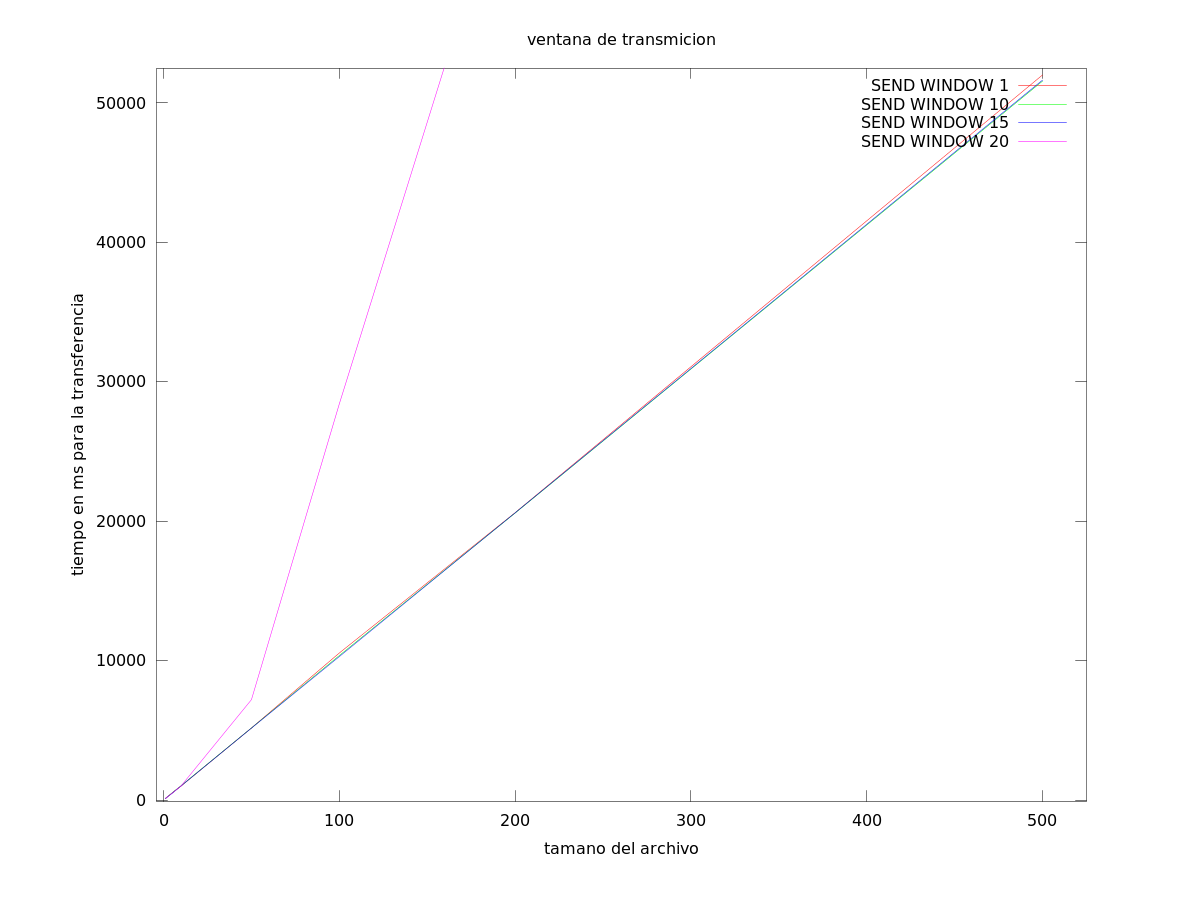
\includegraphics[width=500pt]{./datos/graf.png}
          \caption{Tiempo de transmisión}
          \label{fig:tt}
\end{figure}

\clearpage
\indent En el gráfico podemos observar como el tiempo de transmisión usando
ventanas de 1, 10 y 15, es muy similar. En cambio, cuando usamos una ventana de
20, es notable la diferencia en el tiempo que tarda en enviarse el
archivo. Esto se debe a la cantidad de timeouts que ocurren al utilizar este tamaño de ventana.\\

\subsection{Velocidad de Transferencia}
\indent En este segundo gráfico presentamos la velocidad de transmisión (en kb\/s) de la transmisión de los archivos, usando SEND\_WINDOWs de 1, 10, 15 y 20.

\begin{figure}[h]
  \centering                                                       
          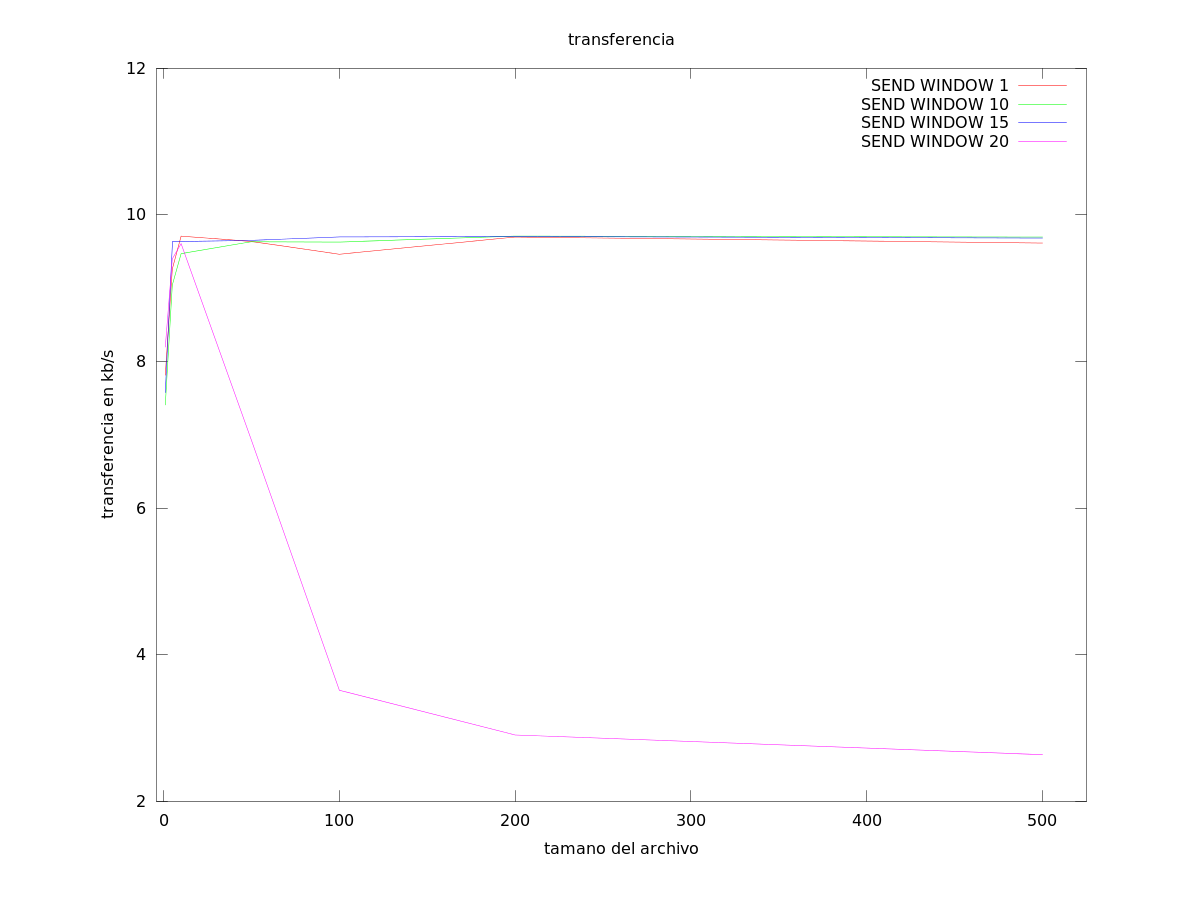
\includegraphics[width=550pt]{./datos/transferencia.png}
          \caption{Tiempo de transmisión}
          \label{fig:vt}
\end{figure}

\clearpage
\indent Al igual que en el gráfico anterior, podemos observar la gran diferencia
que existe en la velocidad de transmisión cuando la ventana de emisión crece.\\
\indent La velocidad se mantiene estable con ventanas de 1,
10 y 15, pero cuando usamos una ventana de 20, la velocidad
tiende a caer mucho a medida de que aumenta el tamaño del archivo.\\
\indent Si comparamos este gráfico con el anterior, se ve claramente como al
ser menor el throughput, el tiempo de transmisión es mucho mayor.\\

\subsection{Cantidad de Timeouts}
\indent En esta sección presentamos la cantidad de timeouts que tuvieron en promedio el envío de los archivos.\\
\begin{center}
   \begin{tabular}{| c | c | c | c | c |}
    \hline
    Tamaño del archivo/SEND\_WINDOW & 1 & 10 & 15 & 20\\
    \hline
    1kb & 0 & 0 & 0 & 0 \\
    \hline
    5kb & 0 & 0 & 0 & 0 \\
    \hline
    10kb & 0 & 0 & 0 & 0\\
    \hline
    50kb & 0 & 0 & 0 & 5\\
    \hline
    100kb & 0 & 0 & 0 & 14\\
    \hline
    200kb & 0 & 0 & 0 & 34\\
    \hline
    500kb & 0 & 0 & 0 & 94\\
    \hline
  \end{tabular}
\end{center}

\indent De igual manera que en las 2 secciones anteriores, podemos observar la gran
diferencia que hay entre las ventanas, en este caso, con respecto a los
timeout.\\
\indent Vemos que con ventanas de 1, 10 y 15, no tuvimos timeout en ninguno de
los archivos que mandamos. En cambio, vemos que con la ventana en 20, los
archivos mas chicos tampoco tuvieron timeout, cuando los archivos mas grandes
empiezan a presentar cada vez mas timeouts. Los timeouts se dan ya que los paquetes encolados en la cola de retransmisión del emisor se les acaba el $RETRANSMISSION\_TIMEOUT$ dado que los acks que se reciben del receptor no llegan lo suficientemente rápido para evitar que se acabe dicho tiempo para el paquete. Si seguimos aumentando el send window a tamaños mayores a 20 solo empeoraríamos la perfomance ya que al producirse un timeout se aplica una política de retransmisión de GoBackN lo que implica que una mayor cantidad de paquetes se deben retransmitir.\\

%\subsection{Tiempo de transmisión}
%\indent En el gráfico podemos observar como el tiempo de transmisión usando
%ventanas de 1, 10 y 15, es muy similar. En cambio, cuando usamos una ventana de
%20, es notable la diferencia en el tiempo que tarda en enviarse el
%archivo. Esto se debe a la cantidad de timeouts que ocurren al utilizar este tamaño de ventana.\\
%
%\subsection{Velocidad de Transferencia}
%\indent Al igual que en el gráfico anterior, podemos observar la gran diferencia
%que existe en la velocidad de transmisión cuando la ventana de emisión crece.\\
%\indent La velocidad se mantiene estable con ventanas de 1,
%10 y 15, pero cuando usamos una ventana de 20, la velocidad
%tiende a caer mucho a medida de que aumenta el tamaño del archivo.\\
%\indent Si comparamos este gráfico con el anterior, se ve claramente como al
%ser menor el throughput, el tiempo de transmisión es mucho mayor.\\
%
%\subsection{Cantidad de TimeOut}
%\indent Al igual que en las 2 secciones anteriores, podemos observar la gran
%diferencia que hay entre las ventanas, en este caso, con respecto a los
%timeout.\\
%\indent Vemos que con ventanas de 1, 10 y 15, no tuvimos timeout en ninguno de
%los archivos que mandamos. En cambio, vemos que con la ventana en 20, los
%archivos mas chicos tampoco tuvieron timeout, cuando los archivos mas grandes
%empiezan a presentar cada vez mas timeouts. Los timeouts se dan ya que los paquetes encolados en el buffer del emisor se les acaba el ttl dado que los acks que se reciben del receptor no llegan lo suficientemente rápido para evitar que se acabe dicho tiempo para el paquete. Si seguimos aumentando el send window a tamaños mayores a 20 solo empeoraríamos la perfomance ya que al producirse un timeout se aplica una política de retransmisión de GoBackN lo que implica que una mayor cantidad de paquetes se deben retransmitir.
